%\setRL
%\pagenumbering{arabic} 



\subsection{
انرژی خمش بر حسب زاویه‌ی دوسطحی
}
 شبکه‌ی ۲ بعدی مثلثی تختی را فرض کنید که طول تمام اضلاع آن 
$a$
 است. در صورتی که صفحه خم شود می‌توان انرژی خم شدن آن را بر حسب بردار عمود بر هر مثلث تعریف کرد،
\begin{equation}
E_b^{discrete}=\frac{1}{2}\epsilon_b\sum_{\langle\alpha,\beta\rangle}|n_\alpha-n_\beta|^2=\epsilon_b\sum_{\langle\alpha,\beta\rangle}\left(1-n_\alpha\cdot n_\beta\right)
\label{eq:bending}
\end{equation}
در اینجا جمع روی تمام جفت‌های 
$n_\alpha$
و 
$n_\beta$ 
است که همسایه‌ی یکدیگر هستند. برای بدست‌ آوردن حد پیوسته‌ فرض می‌کنیم که سطح غشا با پارامتر 
$x(\sigma_i)$
نگاشت شده و محورهای مختصات به صورت 
$e_i=\partial_ix$
تعریف شده که در نتیجه منجر به تعریف متریک و ساختار بنیادی دوم\LTRfootnote{second fundamental form}
 به ترتیب به صورت 
$g_{ij}=e_i\cdot e_j$
و
$\Omega_{ij}=e_i\cdot\partial_jn$
تعریف می‌شود 
\cite{DubrovinModernGeometry}.
 در حد پیوسته اختلاف برداری 
$n_\alpha-n_\beta$
را به صورت گرادیان میدان برداری نوشته می‌شود
\begin{equation}
E_b=\frac{1}{2}\epsilon_b\int dSg^{ij}\partial_in\cdot\partial_jn
%\label{eq:bending}
\end{equation}
با جایگذاری 
$\partial_in\Omega_i^ke_k$
می‌توانیم انرژی خمش را بر حسب 
$\Omega_{ij}$
تعریف کنیم
\begin{equation}
E_b=\frac{1}{2}\epsilon_b\int dSg^{ij}g^{kl}\Omega_{ik}\Omega_{jl}
%\label{eq:bending}
\end{equation}
با استفاده از دو رابطه‌ی 
\begin{equation}
\begin{aligned}
&\epsilon^{il}\epsilon_{jk}=\delta_j^i\delta_k^l-\delta_k^i\delta_j^l\\
&g^{ij}g^{kl}=g^{ik}g^{jl}+\epsilon^{il}\epsilon_{mn}g^{mj}g^{nk}
\end{aligned}
\end{equation}
انتگرالده را به شکل زیر بازنویسی می‌کنیم،
\begin{equation}
\begin{aligned}
g^{ij}g^{kl}\Omega_{ik}\Omega_{jl}&=(g^{ik}\Omega_{ik})^2+\epsilon^{il}\epsilon_{mn}g^{mj}\Omega_{jl}g^{nk}\Omega_{ik}\\
&=(\Omega_i^i)^2+\epsilon^{il}\epsilon_{mn}\Omega_l^m\Omega_i^n=H-2K
\end{aligned}
\end{equation}
که در محاسبات فوق رد\LTRfootnote{Trace}
 و دترمینان ماتریس فرم بنیادی دوم را با خمش متوسط و خمش گاووسی جایگزاری کردیم،
\begin{equation}
\begin{aligned}
H&=tr\{\Omega_k^i\}\\
K&=\det\{\Omega_k^i\}
\end{aligned}
\end{equation} 
که همان انرژی هلفریش است زمانی که سختی خمش و سختی گوسی قرینه‌ی یکدیگر باشند. اینجا نشان دادیم که با تعریف یک ضریف همبستگی میان مثلث‌های همسایه می‌توانیم رفتار انرژی خمش هلفریش را در سیستم ایجاد کنیم. برای یافتن رابطه‌ی بین ضریب همبستگی مثلث‌های شبکه و سختی خمش هلفریش فرض می‌کنیم استوانه‌ای به طول نامتنهای داریم که انرژی خمش یک نوار از آن به ضخامت
$a$
و شعاع
$R$
به شکل زیر محاسبه می‌شود:
\begin{equation}
\begin{aligned}
E_{continuum}&=\frac{1}{2}\int \kappa H^2dS \\
&=\frac{1}{2}a\kappa\int \frac{1}{R^2}d\ell \\
&=\pi\kappa\frac{a}{R}
\end{aligned}
\label{eq:cylindercontinuum}
\end{equation} 

\begin{figure}[h]
\begin{center}
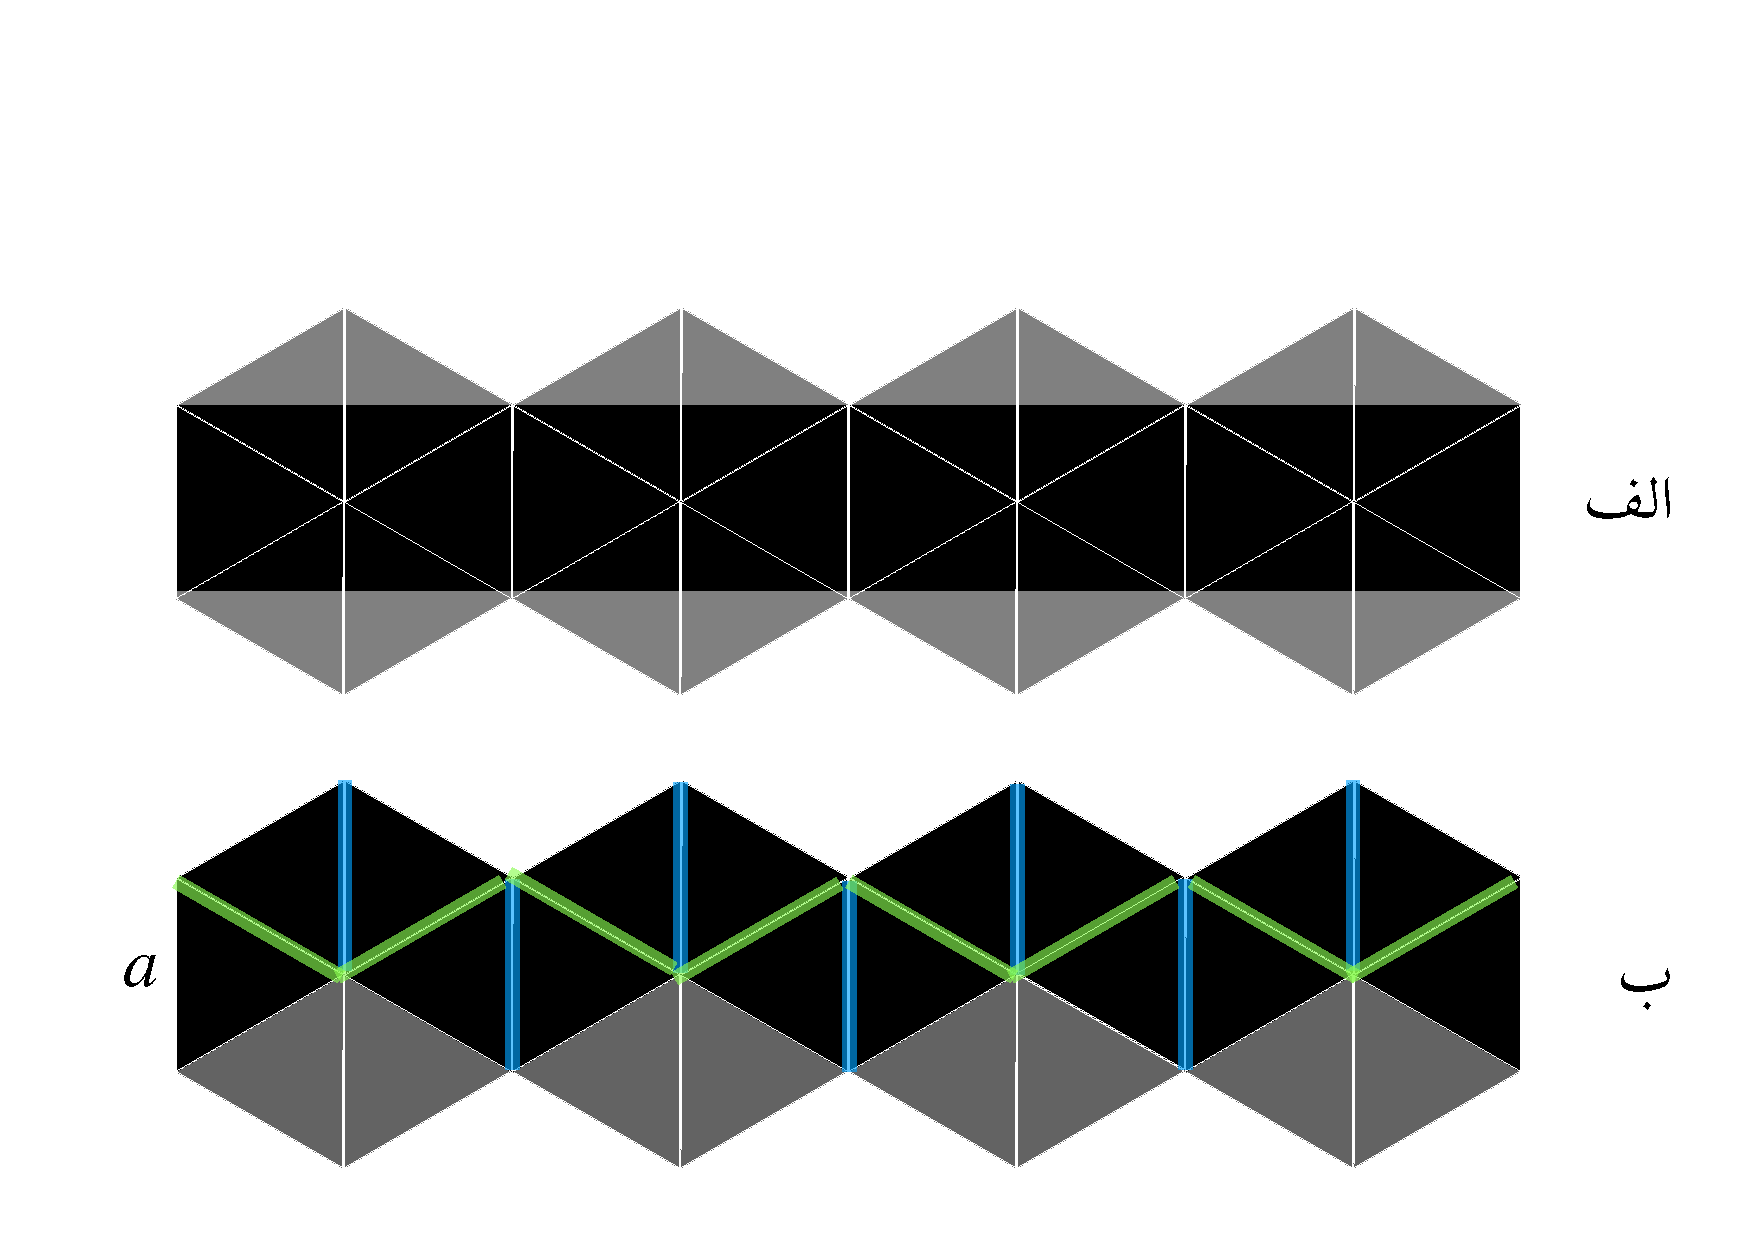
\includegraphics[width=6in]{\MemDiscr/Pics/cylindermesh.pages.pdf}
\caption{
الف، و ب، هر دو نواری از یک شبکه‌ی مثلثی را نشان می‌دهند که هر دو از تعداد یکسان مثلث تشکیل شده‌اند. 
}
\label{fig:cylindermesh}
\end{center}
\end{figure}



ژینوس استوانه برابر ۱ است در نتیجه‌ در محاسبه‌ی انرژي خمش سهمی نخواهد داشت. حال فرض کنید که سطح استوانه را با مثلث (شبکه‌ی نقاط با درجه‌ی ۶) پوشاندیم. شکل
\ref{fig:cylindermesh}
الف، چنین نواری را نشان می‌دهد. اگر فرض کنیم که مثلث‌های نصف شده در بالا و پایین نوار را جابجا کنیم تا مثلث‌های کامل تشکیل شود با شکل
\ref{fig:cylindermesh}
ب، رو برو می‌شویم. اگر این نوار را به دور یک استوانه ببندیم مثلث‌هایی که ضلع مشترک آبی رنگ دارند با یکدیگر زاویه می‌سازند در صورتی که مثلث‌هایی که اضلع مشترک  سبز دارند با یکدیگر زاویه‌ی ۱۸۰ درجه تشکیل می‌دهند. فرض کنیم که طول اضلاع مثلث‌های متساوی الاضلاع 
$a$
 باشد و نوار توسط 
 $N$
 مثلث پوشانده می‌شود. زاویه‌ی میان مثلث‌هایی که ضلع آبی مشترک دارند،
 $\pi\frac{N-2}{N}$
بوده که در نتیجه زاویه‌ی میان بردار‌های عمود به آنها،
 $\pi(1-\frac{N-2}{N})$
خواهد بود. با فرض اینکه تعداد مثلث‌ها به اندازه‌ی کافی بزرگ باشد، انرژی چنین چیدمانی

\begin{equation}
\begin{aligned}
E_{discrete}&=\epsilon_b\sum_{<\alpha,\beta>}\left[1-\cos(\theta_{\alpha,\beta})\right]\\
&=2N\epsilon_b\left[1-\cos\left(\pi(1-\frac{N-2}{N})\right)\right]\\
&=2N\epsilon_b\left[1-\left(1-\frac{1}{2}\left(\pi(\frac{2}{N}\right)^2\right)\right]\\
&=N\epsilon_b\left[\frac{\pi^2}{2}\left(\frac{2}{N}\right)^2\right]\\
&=\frac{4\pi^2}{N}\epsilon_b
\end{aligned}
\label{eq:cylinderdiscrete}
\end{equation} 
در حد 
$N$
های خیلی بزرگ معادله‌ی 
\ref{eq:cylinderdiscrete}
 و 
\ref{eq:cylindercontinuum}
باید پاسخ یکسان داشته باشند. از طرفی محیط سطح مقطع دایره‌ای استوانه با تعداد مثلث‌ها و طول ضلع آن رابطه دارد،
\begin{equation}
\begin{aligned}
2 \pi R &= \frac{N}{2}\frac{\sqrt3}{2}a\\
\frac{a}{R}&=\frac{8}{\sqrt3}\frac{\pi}{N}
\end{aligned}
\label{eq:cylinderdiscretisation}
\end{equation} 
برابر قرار دادن انرژي حد پیوسته و گسسته و جایگاذاری نسبت ضلع مثلث به شعاع استوانه از معادله بالا ما را به رابطه‌ی میان سختی خمش هلفریش و ضریب جفت شدگی مثلث‌ها می‌رساند:
\begin{equation}
\begin{aligned}
\pi\kappa\frac{a}{R}&=4\frac{\pi^2}{N}\epsilon_b\\
\pi\kappa\frac{8}{\sqrt3}\frac{\pi}{N}&=4\frac{\pi^2}{N}\epsilon_b\\
\kappa&=\frac{\sqrt{3}}{2}\epsilon_b
\end{aligned}
\label{eq:epsilonkappa}
\end{equation} 




.
 
 
 
 
 
 
 
 
 
 
 
 
 
 
 